
\section{Traditioneller Anwendungsfall (Systemanwendungsfall)}

\begin{tcolorbox}
    Ein \textbf{Systemanwendungsfall} (auch \textit{System Use Case} oder \textit{Traditioneller Anwendungsfall}
    ist ``ein Anwendungsfall, der speziell das für außen stehende Akteure (Benutzer oder Nachbarsysteme) wahrnehmbare Verhalten eines (Hard-/Software-) Systems beschreibt`` (\cite[361]{Oes05}).\\
\end{tcolorbox}

\noindent
Damit erweitern Systemanwendungsfälle die \textbf{Geschäftsvorfälle} unter Berücksichtigung der Implementierung.\\

\noindent
Um Systemanwendungsfälle zu erarbeiten, können die Anforderungen zunächst informell festgehalten und dann mit zunehmendem Detailierungsgrad ausgearbeitet werden (s. Abbildung~\ref{fig:systemusecase}):

\begin{enumerate}
    \item \textit{High-Level}: Titel, Zusammenfassung einzelner Schritte
    \item \textit{informell}: Ausarbeitung der einzelnen Schritte
    \item \textit{formell}: Ausarbeitung der informellen Version unter Berücksichtigung der beteiligten Systeme und der Implementierung
\end{enumerate}

\noindent
\textit{Wedemann} empfiehlt, in der Anforderungsphase keine formellen Anwendungsfälle zu erstellen, da diese bereits sehr umfangreich und detailliert ausfallen können.
Deshalb sollte diese erst in der Analysephase unter zuhilfenahme von Aktivitätsdiagrammen, Ablaufdiagrammen und Domänenmodellen erstellt werden. (vgl. \cite[71]{Wed09}).

\begin{figure}
    \centering
    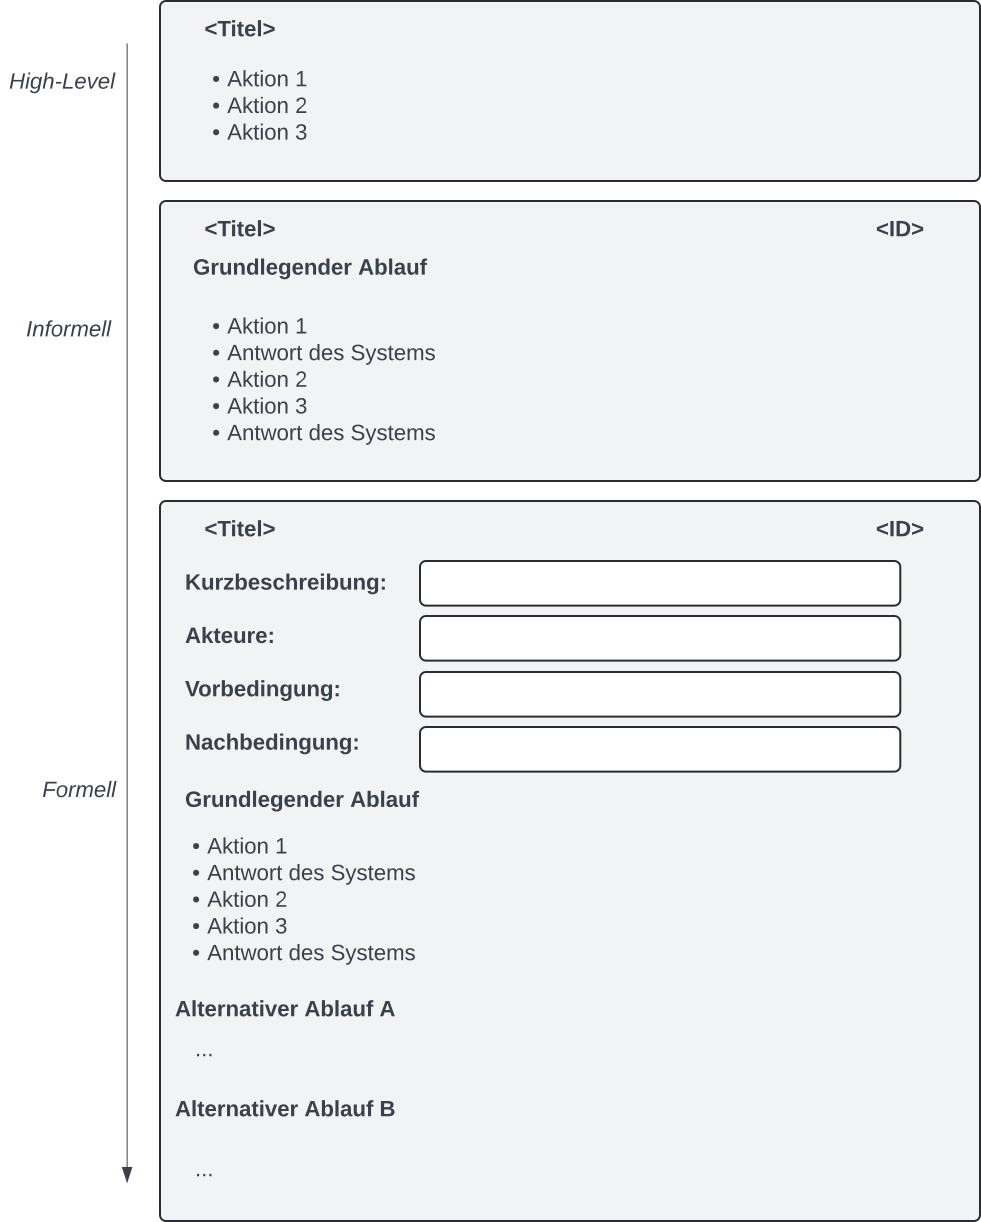
\includegraphics[scale=0.4]{chapters/Anhang/CheatSheets/img/systemusecase}
    \caption{Verschiedene Evolutionsstufen eines Systemanwendungsfalls. (Quelle: in Anlehnung an \cite[Abb. 4.6, 4.7, 4.8]{Wed09})}
    \label{fig:systemusecase}
\end{figure}